\section{Nuclear Power in the UK}


\begin{figure}[htbp]
  \begin{center}
    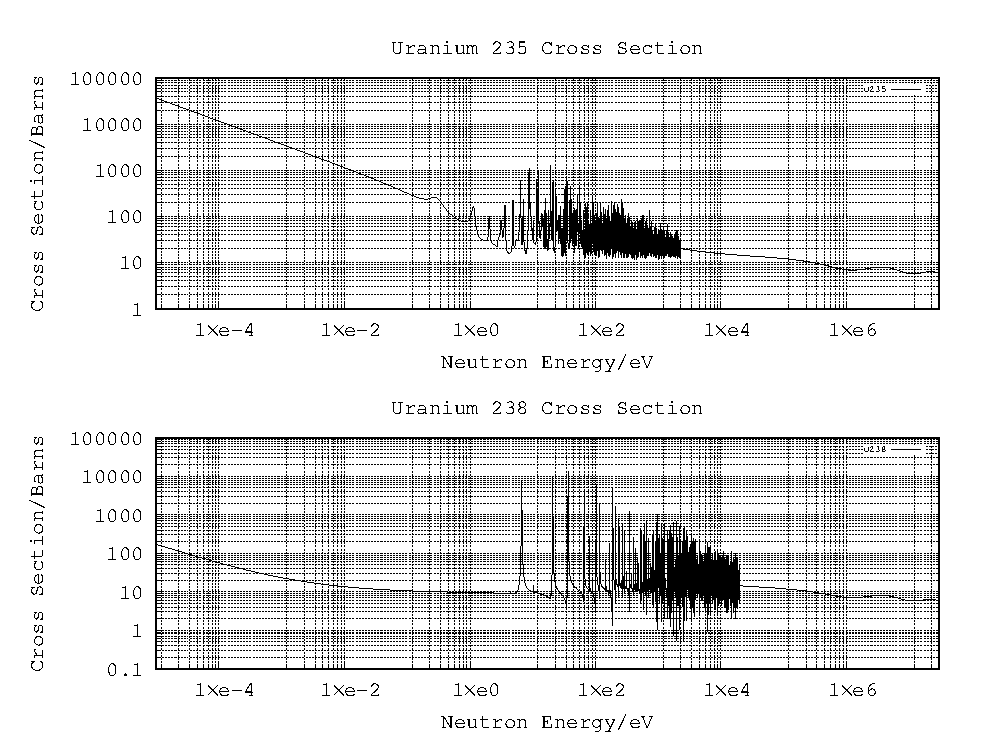
\includegraphics{chapters/introduction/plots/uranium_cross_section/u_xs}%
    \caption{Graph caption}
    \label{graph:graph1}
  \end{center}
\end{figure}




\subsection{Generation I Reactors}

Magnox type reactors were the first used in the United Kingdom.  These reactors used natural Uranium as a fuel and were carefully designed to produce energy despite using an unenriched fuel.  Graphite was used as a moderator, and the low neutron capture cross section of the Magnox cladding allowed a nuclear reaction to occur despite the fuel not being enriched.

In all there were 11 Magnox power stations built in the UK with 26 reactors in total.  All have now shut down and the last, Wylfa, closed in 2015.


\subsection{Generation II Reactors}

There are 15 reactors currently operating in the UK, and they are all Generation II reactors.  Of these, 14 are Advanced Gas Reactors and 1, Sizewell B, is a Pressurised Water Reactor.

\begin{figure}[tbp]
  \begin{center}
    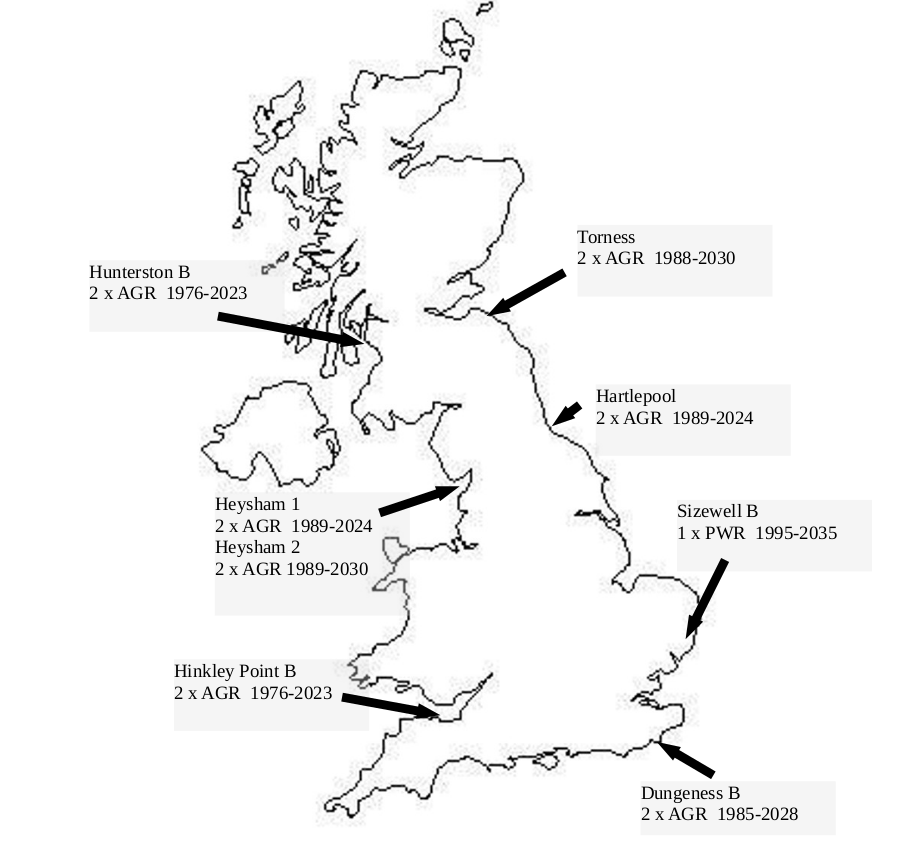
\includegraphics[width=12.0cm]{chapters/introduction/images/remaining_plants.png}
    \captionsetup{font={it}}
    \caption{Remaining reactor locations in the UK}
    \label{fig:electricityusagesuk}
  \end{center}
\end{figure}




\subsection{Generation III Reactors}

There are no Generation III reactors operating in the UK.  The first was built in Japan, and the type of reactor installed was an Advanced Boiling Water Reactor (ABWR) built in 1996 in Japan.  Two sites have been proposed for the UK for the Generation III Hualong One type PWR reactor power plant:  Sizewell C and Bradwell B, and the expected opening date is between 2030-2035.   The final type of operational reactor of this generation is the Russian fast breeder reactor, a single reactor of its type, built in Zarechny, Russia. 




\section{An Approaching Energy Gap for the UK}

Since Calder Hall, the first commercial nuclear power plant, opened in 1956, the demand on electrical power generation in the UK has tripled.  There is now a reliance on cheap and clean power from nuclear reactors as these provide a quarter of our electricity.  There are sixteen reactors operational in the UK:  the Magnox reactor at Wylfa and the fourteen AGR reactors are due to be decommissioned by 2023\cite{gen4}, and the remaining PWR reactor, Sizewell B, is expected to remain operational until 2035\cite{gen4}.

\begin{figure}[tbp]
  \begin{center}
    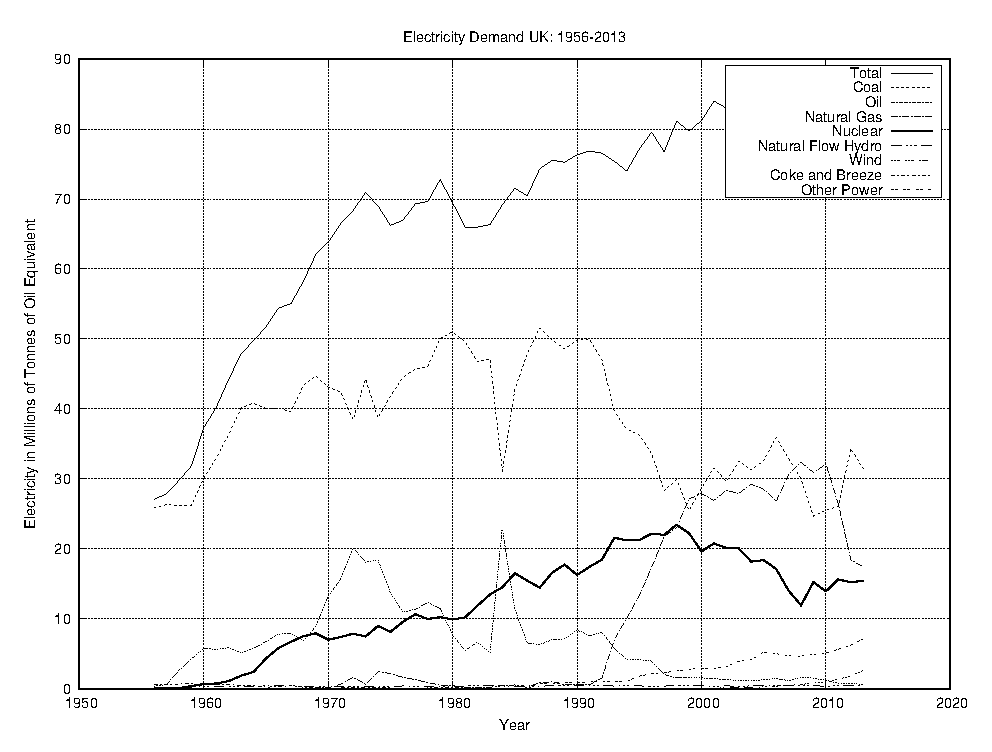
\includegraphics[width=15.0cm]{chapters/introduction/plots/elec_demand/elec_demand.eps}
    \captionsetup{font={it}}
    \caption{Electricity in Millions of Tonnes of Oil Equivalent}
    \label{fig:electricityusagesuk}
  \end{center}
\end{figure}

There is an obvious concern that within the next ten years the UK will lose a sizeable proportion of its electricity generation capabilities, however, there are proposals to remedy this.  EDF have planned to build two new reactors at the Hinkley Point site in Somerset.  Hinkley Point C will contain two Areva NP designed Gen III+ EPR reactors.  Many advanced materials, including a variety of types of Austenitic Stainless Steel, will be used in the construction of these reactors. 

The physical stresses subjected to the Gen IV reactors will go beyond those that are currently being built.  There will be higher radiation doses and faster, more damaging neutrons.  Coolant temperatures will be higher to either give better thermodynamic efficiency or open the route to creating hydrogen directly as a fuel.  Novel coolants such as lead and sodium, each with their own challenges to overcome, are also being considered.



\subsection{Proposed Generation III+ Nuclear Power Plants}

Two Generation III+ reactors are under construction in the UK: Hinkley Point C 1 and C 2.  These reactors are Areva European Pressurized Reactors (EPR), which are PWRs, and the proposed opening years are 2025 and 2026 respectively.




\subsubsection{Areva EPR}

The 1.6GW Areva EPR design has four primary loops transferring heat by pressurised water from the reactor to heat exchangers.  It requires Uranium enriched to 5% 235U in the form of Uranium Oxide Pellets.  The inlet temperature is 295.6OC and the outlet temperature is 329.8OC.

There are 241 fuels assemblies, each containing 265 fuel rods giving a total of 63865 rods.  The fuel rod cladding is made from 316 stainless steel and has an inner diameter of 7.72mm and an outer diameter of 9.68mm.

The materials used to construct the control rod drive mechanisms includes 410 stainless steel and 304 stainless steel.


\subsubsection{Westinghouse AP1000}

The 1.1GW Westinghouse AP1000 degsign is a pressurised water reactor with two primary loops transferring heat from the reactors to heat excahngers.  An enriched Uranium Dioxide fuel, up to 5% 235U, is clad in Zirlo (proprietary Zirconium alloy).  

The inlet temperature is 279.4oC and the outlet temperature is 324.7oC which is close to the temperature range of the EPR reactor.  The composition of the control rod absorber material includes 304 Stainless Steel.









Although work has not started, at the time of writing, several sites have been acquired with the aim of building new nuclear power stations.  There are five sites and three reactor designs\cite{ocw01}:
\begin{itemize}
\item Hinkley Point: two Areva EPRs (EDF Energy)
\item Sizewell: two Areva EPRs (EDF Energy)
\item Wylfa: 2-3 Hitachi ABWRs (Horizon Nuclear Power)
\item Oldbury: 2-3 Hitachi ABWRs (Horizon Nuclear Power)
\item Sellafield: 3 Westinghouse AP1000s (NuGeneration)
\ldots 
\end{itemize}






\subsection{Generation IV Proposed Designs}






\subsubsection{Lead-cooled Fast Reactors}

One example of the next generation reactor designs is ELSY: the European Lead Fast Reactor.  It is a fast neutron reactor and this benefits from a lead coolant as lead has a low reaction cross section and the maximum energy lost per neutron-coolant atom collision is low.  The Lead coolant will be at a temperature of 400oC to 480oC\cite{elsy01} and will weigh 9,000 tons.  The challenge for engineers is to develop materials that can survive such extreme conditions, including the corrosiveness of the liquid lead and the high flux of fast neutrons.   (5).

\begin{figure}[tbp]
  \begin{center}
    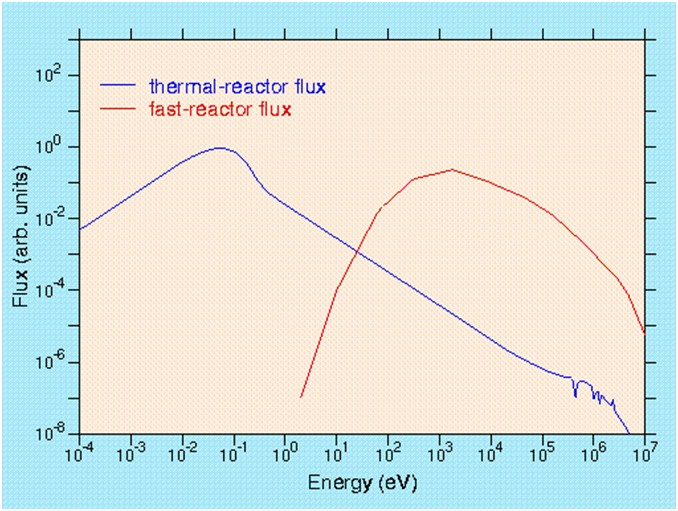
\includegraphics[width=7.0cm]{chapters/introduction/images/reactor-flux.png}
    \caption{Graph caption}
    \label{image:flux1}
  \end{center}
\end{figure}


\subsubsection{Gas Cooled Fast Reactors}

Very high outlet temperatures can be achieved for GFRs, with the temperature of the gas coolant ranging from 490oC to 850oC (6) and this requires advanced materials that can withstand temperatures as high while under high energy neutron flux.  Unlike LFRs and SCWRs, the coolant is inert, leaving engineers to overcome high temperatures and irradiation damage. 



\subsubsection{Sodium Cooled Fast Reactors}




\subsubsection{Very High Temperature Reactors}




\textbf{Super-Critical Water Reactors (SCWR)}

At 647K and a pressure of 22.1MPa (approximately 218 atmospheres), becomes supercritical which is neither a liquid or a gas\cite{advancedbiomass}.

\begin{figure}[tbp]
  \begin{center}
    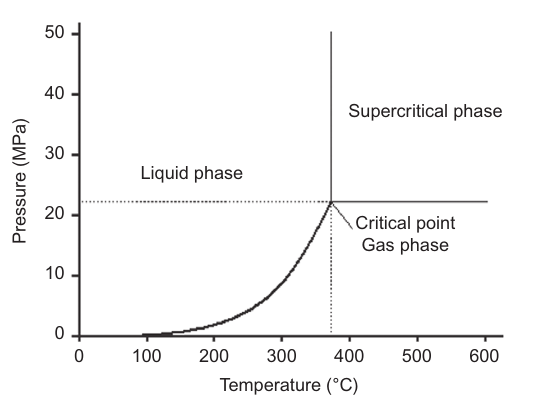
\includegraphics[width=7.0cm]{chapters/introduction/images/water_phase_diagram.png}
    \caption{Graph caption}
    \label{image:flux1}
  \end{center}
\end{figure}


Supercritical water exists above 374oC and 22.1MPa, and in this state water has a higher thermodynamic efficiency.  The design of the nuclear power plant is also simplified as there is no phase change of the water, so a condenser is not needed.  The SCWR is the only GEN IV reactor design that uses water as the coolant\cite{gen4}.  The economic benefits have already been seen in SCW fossil fuel power stations, and it is incorporated in GenIV water cooled fast and thermal reactors.  The combination of supercritical water chemistry and irradiation damage must be considered, as well as higher temperature and pressure.

PWR 288-325oC 15.2 MPa\cite{ocw01}

BWR 278-287oC 7.1MPa\cite{ocw02}



\subsubsection{Molten Salt Reactors}





\subsubsection{Experimental Fusion Reactors}

Nuclear Fusion is a very attractive technology and could be the answer to all of our energy problems.  Much work is being invested in developing this technology and the ITER (International Thermonuclear Experimental Reactor) has been designed to output more energy than is required to start the fusion reaction.  The process of fusion combines two isotopes of hydrogen and leaves helium and fast neutrons.  As neutrons have no charge, they can penetrate shielding causing damage as they lose energy through nuclear interactions.   Any atoms they interact with have a chance to capture the neutron and become unstable.

\begin{equation}
_{1}D^{2} + _{1}T^{3} \to _{2}He^{4} (3.5MeV) + _{0}n^{2} (14.1MeV)
\end{equation}

The fast neutron spectrum for fission reactors ranges from a few eV to a few MeV, whereas the neutrons in a fusion reaction have 2-3 times more energy than the most energetic neutrons from fast fission.  Engineers must develop materials to construct components that will be resilient to this damage, while having a low reaction cross section and being able to withstand other extreme conditions within the reactor.  








